\section{Preprocesamiento de Datos y Justificación Matemática}\label{sec:preprocessing}
 
\subsection{Partición de datos}
El conjunto de datos se particionó en 80\% de entrenamiento y 20\% de prueba, garantizando estratificación respecto a la variable objetivo:
\begin{equation}
X_{train}, X_{test}, y_{train}, y_{test} = \text{split}(X, y; \; p_{test}=0.20, \; \text{stratify}=y)
\label{eq:split}
\end{equation}
con $\text{random\_state}=42$. Las dimensiones resultantes fueron $X_{train} \in \mathbb{R}^{1\,338\,261 \times 15}$ y $X_{test} \in \mathbb{R}^{334\,566 \times 15}$, tras excluir las variables temporales (\texttt{año}, \texttt{dia}) y la variable objetivo del vector de características.
 
\subsection{Imputación}
Los valores faltantes remanentes se imputaron utilizando la mediana de cada variable en el conjunto de entrenamiento, con el fin de mitigar la asimetría de las colas pesadas presentes en variables como el viento y la humedad:
\begin{equation}
\hat{x}_{i,j} = \text{median}\left(\{x_{k,j} : x_{k,j} \neq \text{NaN}, \; k \in \text{train}\}\right)
\label{eq:median}
\end{equation}
 
\subsection{Escalamiento robusto}
Dado que los valores climáticos extremos constituyen señal predictiva legítima y no ruido, se utilizó \texttt{RobustScaler}, que centra los datos mediante la mediana ($Q_2$) y los escala mediante el rango intercuartílico:
\begin{equation}
x'_{i,j} = \frac{x_{i,j} - Q_2(x_{\cdot,j})}{IQR(x_{\cdot,j})}, \quad IQR = Q_3 - Q_1
\label{eq:robust}
\end{equation}
Esta transformación evita que los microclimas extremos distorsionen la topología del espacio vectorial, a diferencia de la estandarización clásica ($z$-score) basada en la media y la desviación estándar, susceptible a colas distributivas largas.
 
El preprocesamiento se encapsuló en un \texttt{Pipeline} de \emph{scikit-learn} compuesto por \texttt{SimpleImputer(strategy='median')} seguido de \texttt{RobustScaler()}, integrado dentro de un \texttt{ColumnTransformer} ajustado exclusivamente sobre $X_{train}$ y aplicado en modo transformación ciega sobre $X_{test}$, evitando la fuga de información estadística entre particiones.
 
\subsection{Reducción de dimensionalidad (PCA)}
Debido a la alta multicolinealidad identificada en el análisis de correlación, se aplicó Análisis de Componentes Principales (PCA) sobre $X_{train}$ escalado. La proyección hacia un subespacio de dimensión $K$ se define como:
\begin{equation}
Z = X' W_K
\label{eq:pca}
\end{equation}
donde $W_K \in \mathbb{R}^{p \times K}$ contiene los $K$ autovectores principales de la matriz de covarianza de $X'$. El número óptimo de componentes se determinó como el mínimo $K$ tal que la varianza acumulada explicada satisface:
\begin{equation}
\sum_{i=1}^{K} \lambda_i \Big/ \sum_{i=1}^{p} \lambda_i \geq 0.95
\label{eq:variance}
\end{equation}
Se obtuvo $K=5$ componentes principales de un total de 15 características originales, reduciendo la dimensionalidad del espacio de características en un 66.7\% mientras se retiene el 95\% de la varianza empírica (Fig. \ref{fig:pca}).
 
\begin{figure}[H]
\centering
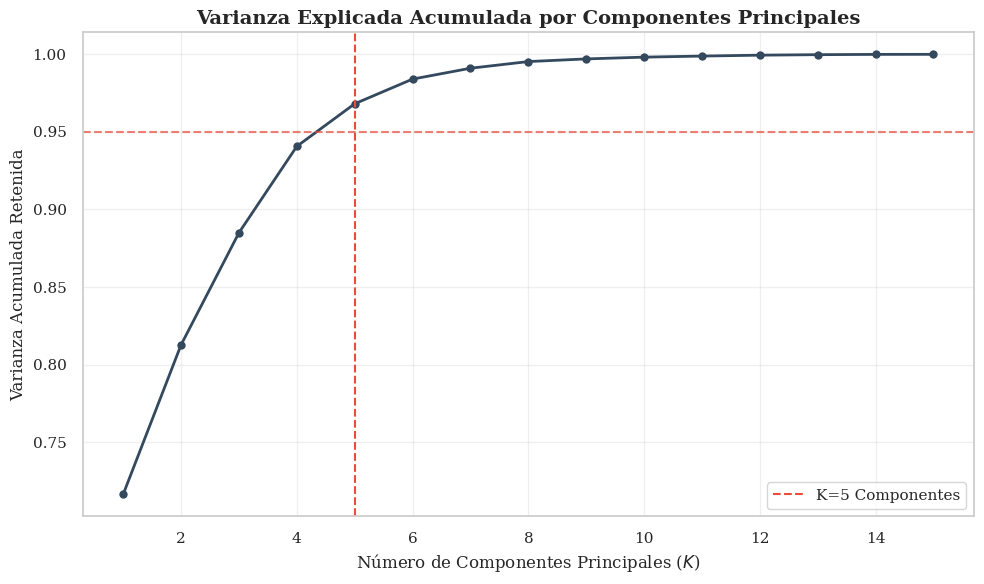
\includegraphics[width=0.90\textwidth]{img/cell13_out1.png}
\caption{Varianza acumulada explicada por componente principal, con el punto de corte $K=5$ para retener el 95\% de la varianza.}
\label{fig:pca}
\end{figure}
 
Se descartaron técnicas de reducción no lineal como \emph{t-SNE}, dado que el objetivo era preservar un mapeo afín de las varianzas continuas útil para un clasificador de particiones ortogonales, propiedad que la no linealidad estocástica no garantiza.